\documentclass[a4paper]{article}

\usepackage{fullpage} % Package to use full page
\usepackage{parskip} % Package to tweak paragraph skipping
\usepackage{tikz} % Package for drawing
\usepackage{amsmath, amssymb}
\usepackage[amsmath, amsthm, thmmarks]{ntheorem}
\usepackage{hyperref}
\usepackage[utf8]{inputenc}
\usepackage[english]{babel}

\theoremstyle{break}
\theoremindent=1cm
\theoremheaderfont{\kern-1cm\normalfont\bfseries}
\theorempreskip{0.4cm}
\theorempostskip{0.4cm}

\newtheorem{theorem}{Theorem}[section]
\newtheorem{definition}{Definition}[section]
\newtheorem{corollary}{Corollary}[theorem]
\newtheorem{lemma}[theorem]{Lemma}


\newcommand{\bib}{???}
\newcommand{\R}{\mathbb{R}}
\newcommand{\Nu}{\mathcal{N}}
\newcommand{\Ra}{\mathcal{R}}
\newcommand{\Exp}{\mathbb{E}}
\newcommand{\Mat}[2]{\mathbb{M}(#1, #2)}
\newcommand{\Part}[2]{\frac{\partial #1}{\partial #2}}

\DeclareMathOperator{\La}{\mathcal{L}}
\DeclareMathOperator{\diag}{diag}
\DeclareMathOperator{\bO}{\mathcal{O}}
\newcommand{\pll}{\parallel}

\title{Mathematics behind Machine Learning Algorithms}
\author{Hubert Beres}
% \date{2018/01/08}

\begin{document}

\maketitle

\section{Introduction}

\subsection{Abstract}
Rough work, to be written in nice English.

Recently we face many problems where objective is to guess a function of multiple variables (features) based on multiple examples (values at particular points).

In this essay:

\begin{enumerate}
    \item describe context of supervised machine learning
    \item introduce multiple linear regression as one of suitable models
    \item derive Moore-Penrose generalised inverse of a matrix as a tool of calculating regression coefficients
    \item motivate usage of non-linear models
    \item Introduce a simple neural network in comparison to a linear model
    \item Discuss difficulties of finding the right parameters for the network, describe stochastic gradient algorithm
\end{enumerate}

\subsection{Machine learning context}

Rough work, to be written in plain English.

\begin{enumerate}
    \item In this essay I focus on functions from multiple real-valued inputs to a single real output (though multiple output variables can be easily generalised to).
    $$ f : \R^n \to \R $$
    
    \item example where we want to fit such function
    
    \item We call a vector $x \in \R^n $ of values in the domain of $f$ a data point or data sample.
    
    \item If we know the value $ y_i = f(x_i) $ \textit{a priori} for certain points $ x_i \in X $ we call the set $X$ a training set and we refer to values $ ( y_i) $ as labels.
    
    \item In mathematical formulation it is often convenient to organise the training set into a matrix $H$ where each data point is represented by a row. Then we gather the labels into a vertical vector $y$. Function $f$ is understood to act on every row of a matrix separately, resulting in a corresponding label, so that
    $$ f(H) = y $$
    
    In most practical applications the number of data samples is much larger than the number of the features so we think about $H$ as a rectangular matrix with more rows than columns.
    
    \item A supervised learning algorithm describes a process of analysing a training set and producing a function $ F : \R^n \to \R $ which approximates $f$ over its domain.
    
    \item The usual way of measuring how well $F$ approximates $f$ is evaluating $F(H)$ and comparing it to the labels $y$.
    It is often convenient to consider a sum of squares of errors made on each sample, which in matrix notation is equivalent to:
    $$ \| F(H) - f(H) \|^2 = \| F(H) - y \|^2 $$
    The goal of the algorithm is then to find $F$ that minimises the above value, referred to as training error.
    
    \item Most supervised algorithms presuppose certain form of $F$, parameterised by a vector $ \omega \in \Omega$. We write $ F(\omega; x) $ meaning that once parameters are set, $F$ can be evaluated on an arbitrary point $x$ of its domain. In such parameterised model the goal of an algorithm is to find parameters $\omega$ that result in minimal training error. We often refer to the process of finding $ \omega $ as training the model.

    \item Although during the training only training set is available to measure error on, at the end of the day we'd like $F$ to approximate $f$ also on data points that are similar to the ones in $H$ but not identical.
    It comes out that due to random variation in the test sample, "simpler" models with slightly higher test error generalise better than the ones that tried to fit the noisy data more closely rather than following general patterns. The issue of poor generalisation of too "complicated" models is known as overfitting.
    
    \item As a rule of thumb a model is more likely to overfit when it has more parameters in $ \omega $. Among models with the same parameter space $ \Omega $ the ones with smaller values of parameters generalise better. A good measure of that size is the norm of parameter vector: $ \| \omega \| $.
    % this is a bold oversimplification but... I don't really want to go there as I'm short on space anyway.
    % it may be beneficial to include classic polynomial overfitting example here...
\begin{figure}[!htbp]
\begin{center}
    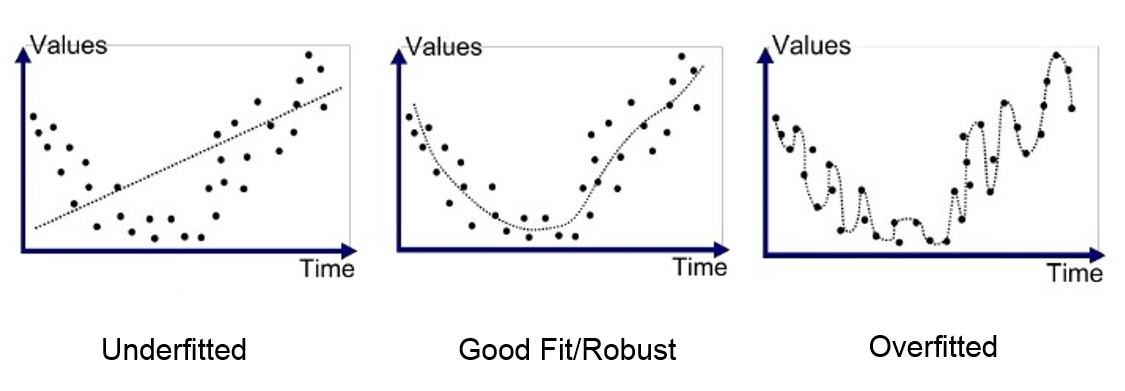
\includegraphics[width=8cm]{overfit_poly.png}
\end{center}
\caption{Classic overfit example that may be worth discussing.}\label{overfit}
\end{figure} 
    
\end{enumerate}

With this motivation we first look into the simplest parametric model: linear regression.

\begin{equation}
    \label{def}
        \| T w - l \| = \inf\limits_{x \in \R^n} \| T x - l \|
\end{equation}
    
\begin{definition}[Multiple Regression]
    Given a real-valued $ n \times m$ matrix $T$ and a n-vector $l$ a Multiple Regression Model is a linear map $f \in \mathcal{L} ( \R ^n, \R)$ represented by a $ 1 \times n$ matrix $w$ such that
    \begin{equation}\label{def2}
        \| T w - l \| = \inf\limits_{x \in \R^n} \| T x - l \|
    \end{equation}
\end{definition}
A similar definition can be written for multivariate linear regression where $ f \in \mathcal{L} ( \R ^n, \R^m)$. Finding the optimal parameters in such case is performed separately for every output variable. Hence, for the sake of simplicity we'll focus on real-valued functions.

In the following two sections I explore algebraic background that shows $ w $ can indeed be found and develop tools for computing it, given a matrix $T$ representing the training set and the vector of labels $l$.

\section{Facts from Linear Algebra}

We start by stating several theorems that are parts of the curricula for the second year or are closely related to the familiar notions of vector (sub)space, range and null space. The first result provides a useful way of decomposing a vector into two components, exactly one lying inside a vector subspace. Uniqueness of such decomposition will be useful when showing uniqueness of our optimal solution for the regression problem.

This section is a selection of statements from introduction in \bib adjusted to knowledge from Algebra courses. Proofs are inspired there except for \ref{lem:double_perp} which is my own improvisation.

\subsection{Conventions}
\begin{enumerate}
    \item Vectors are by default column vectors,
    \item Matrices are real,
    \item Orthogonal vectors are denoted by $ v \perp w$
    \item $\Nu(H)$ resp. $\Ra(H)$ denote the null space resp. the range of a matrix $H$.
\end{enumerate}

\subsection{Orthogonal decomposition}
As introduced in the Geometry module, we define two vectors as perpendicular (denoted by $ a \perp b$) if and only if their scalar product is 0. Given a vector subspace $V \in \R^n$ we can think about vectors perpendicular to all its elements and denote them as $z \perp V$. We call a set of all such vectors the orthogonal complement of $V$:
$$ V^\perp := \{ v \in \R^n : v \perp V\} $$
Notice that $V^\perp \cap V = \{0\}$ and that $V^\perp$ is itself a vector subspace since scalar product is linear. The following theorem provides a widely useful decomposition of an arbitrary vector:

\begin{theorem}[Orthogonal decomposition] \label{thm:projection}
    Let $z \in \R^n$ and $V \subset \R^n$ be a vector subspace. Then
    There exist unique $z_\perp \in V^\perp$ and $z_\pll \in V$ such that  
    \begin{equation}
        z = z_\perp + z_\pll
    \end{equation}
\end{theorem}

\begin{proof}
    The proof has been presented in Geometry module.
\end{proof}

As we are interested only in finite-dimensional vector spaces the dimension formula
\begin{equation}\label{eq:dim_formula}
    dim(U + V) = dim(U) + dim(V) - dim( U \cap V)
\end{equation}
allows us to conclude an important property of the complement defined above:

\begin{lemma}\label{lem:double_perp}
    If $W$ is a finite-dimensional vector space and $V$ is its subspace then
    $$ V = (V^\perp)^\perp $$
\end{lemma}

\begin{proof}
    Pick an $x \in V$. By definition $ V^\perp = \{ y \in W : y \perp x \text{for all } x \in V \}$ hence for every $y \in V^\perp $ there is $x \perp y$. On the other hand $ (V^\perp)^\perp = \{ x \in W : x \perp y \text{for all } y \in V^\perp \}$ so $x \in (V^\perp)^\perp$, i.e.
    $$ V \subset (V^\perp)^\perp$$

    Now as $W = V + V^\perp$ is finite-dimensional, let $dim(W) = n$ and $dim(V) = k$. 
    As we know that $V \cap V^\perp = \{0\}$, by the dimension formula (\ref{eq:dim_formula}) we have
    $$ dim(V^\perp) = dim(W) - dim(V) = n - k $$
    We can apply the dimension formula again, noting that $ V^\perp \cap (V^\perp)^\perp = \{0\} $ to get:
    $$ dim((V^\perp)^\perp) = dim(W) - dim(V^\perp) = n - n + k = k $$

    We have shown $ V \subset (V^\perp)^\perp$ and $ dim(V) = dim((V^\perp)^\perp)$,
    hence $ V = (V^\perp)^\perp$.
\end{proof}

Once we have defined an orthogonal complement it comes handy to relate them with notions of null space and range.
The key result is a characterisation of a null space presented below:

\begin{theorem} \label{thm:charact_nullspace}
    For any matrix $H \in \Mat{n}{m}$ the null space of $H$ is equal to perpendicular complement of $H^T$ in $\R^m$, i.e.
    $$\Nu(H) = \Ra^\perp(H^T)$$
\end{theorem}

\begin{proof}
    Pick any $x \in \Nu(H)$ we have $H x = 0$, implying $ y^T H x = 0$ for any $y \in \R^n$. Now
    $$  y^T H x = (H^T y )^T x = 0$$
    which means that $x$ is orthogonal to all vectors of the form $ H^T y $, i.e. $ x \perp \Ra(H^T)$, showing $ \Nu(H) \subset \Ra^\perp(H^T)$. To see the other inclusion take $ y \in \Ra(H^T) $ and conclude from the above equation that $ H x = 0$, i.e. $ x \in \Nu(H)$.
\end{proof}
A very similar proof leads to a complementary statement:
\begin{corollary} \label{cor:charact_range}
    $$\Nu^\perp(H) = \Ra(H^T)$$
\end{corollary}

Moreover, Theorem \ref{thm:charact_nullspace} provides another useful way of decomposing vectors in $\R^n$, this time with respect to their properties related to a matrix $H$.
\begin{corollary}
    For every vector $z \in R^n$ there exists unique decomposition where $z_\Ra \in \Ra(H)$ and $z_\Nu \in \Nu(H^T)$:
    $$z = z_\Ra + z_\Nu$$
\end{corollary}

\begin{proof}
    Given $ z \in \R^n$  apply theorem \ref{thm:projection} with $\Ra(H)$ as the vector subspace to get unique
    $ z = z_\perp + z_\pll$ with $z_\perp \in \Ra^\perp(H)$. By Theorem \ref{thm:charact_nullspace} applied to $H^T$ we get $\Ra^\perp(H) = \Nu(H^T)$, completing the proof as we set $z_\Ra := z_\pll$ and $z_\Nu := z_\perp$.
\end{proof}

\subsection{Symmetric matrices}
We close this section with a few remarks on symmetric matrices and subspaces they generate. The importance of these results comes from the fact that symmetric matrices are always diagonalizable in $\R$ and hence play an important role in finding eigenvalues which come out to be closely related to our regression optimisation problem. 

\begin{lemma} \label{lem:charact_sym_nullspace}
    If $A$ is a symmetric matrix then $\Nu(A) = \Ra^\perp(A)$ and $\Nu^\perp(A) = \Ra(A)$.
\end{lemma}
\begin{proof}
    The claim follows immediately from Theorem \ref{thm:charact_nullspace} when we substitute $A^T = A$.
\end{proof}

\begin{lemma}
Matrices of the form $H^T H$ and $H H^T$ are symmetric for arbitrary $H \in \Mat{n}{m}$.
\end{lemma}
\begin{proof}
    Direct check shows:
    $$(H^T H)^T = H^T (H^T)^T = H^T H \text{ and } (H H^T)^T = H H^T$$~
\end{proof}

\begin{lemma}
    \label{lem:nullspaces_hht}
    For an arbitrary matrix $H$,
    $$\Nu(H) = \Nu(H^T H) \text{ and } \Nu(H^T) = \Nu(H H^T)$$
\end{lemma}

\begin{proof}
    We'll show mutual inclusion for the first equality. To prove that $\Nu(H) \subset \Nu(H^T H)$ pick $x$ such that $H x = 0$. Multiplying both sides by $H^T$ we get
    $$ H^T H x = H^T 0 = 0 $$
    implying $x \in \Nu(H^T H) $.
    To show the other inclusion, pick $x \neq 0$ such that $H^T H x = 0$. Multiply from the right by $x^T$ to get
    $$ x^T H^T H x = (H x)^T H x = \| H x \|^2 = 0 $$
    implying $ H x =0 $ as required.
    
    The second equality of the lemma follows by a similar argument.
\end{proof}

Perhaps the most interesting part of the above proof is the technique of completing a product of matrices to an expression of the form $v^T v = \| v \|^2 $ and then using knowledge about norm of $v$ to reason about its structure.

An immediate corollary of Lemma \ref{lem:nullspaces_hht} provides analogous relationships between ranges:

\begin{corollary}\label{cor:equal_ranges}
    For an arbitrary matrix $H$,
    $$\Ra(H) = \Ra(H H^T) \text{ and } \Ra(H^T) = \Ra(H^T H)$$
\end{corollary}

\begin{proof}
    We use the characterisation of null spaces proven before and compute orthogonal complements of each side. For example
    $$ \Nu(H) = \Ra^\perp (H^T) \text{ and } \Nu(H^T H) = \Ra^\perp ( H^T H )$$
    by Theorem \ref{thm:charact_nullspace}. From the last lemma we have
    $ \Nu(H) = \Nu(H^T H) $ so by the above:
    $$ \Ra^\perp (H^T) = \Ra^\perp ( H^T H ) $$
    or, by Lemma \ref{lem:double_perp}:
    $$ \Ra (H^T) = \Ra( H^T H ) $$
    as required. The other formula follows by a similar argument.
\end{proof}


\section{Moore-Penrose pseudoinverse}
Linear Algebra addresses a fundamental problem of solving a system of linear equations
$$ A x - b = 0$$
by introducing a notion of matrix inverse. If $x$ is a vector of unknown variables and certain conditions are met (including $A$ being a square matrix) one can obtain the solution as: $ x = A^{-1} b $. As our problem of Multivariate Regression is almost identical in structure
$$ \inf \| T x - l \| $$
we would be interested in finding an analogous operation, say $ T \to T^+$ such that $ w = T^+ l$ where $w$ is a vector of coefficients minimising the training error. Unfortunately we cannot use the matrix inverse as in all practical circumstances we expect $T$ to be rectangular (amount of test samples should be much bigger than number of parameters)! On the other hand we don't hope to find an exact solution $ T w = l$ but rather just make the vectors $T w$ and $l$ ``as close as possible" under the standard norm.

This trade-of between precision of the solution and its guaranteed existence motivates defining the Moore-Penrose pseudoinverse.

\subsection{Derivation}
First of all, we should make sure that the operator $T^+$ can be well defined, i.e. that given a multiple regression problem there exists a single vector of "the best" coefficients, minimising the training error.
The following two theorems assure existence of the solution and provide an interesting way of picking the best vector among those yielding the same error.

Proofs in this section are inspired on \bib, though significant changes and simplifications have been introduced.

\begin{theorem}\label{thm:regression_existence}
With a matrix $H \in \Mat{n}{m}$ and $z \in \R^n$ the set
\begin{equation*}
    X := \{ x \in \R^n : \| z - H x \| = \inf\limits_{y \in \R^n} \| z - H y \| \}
\end{equation*}
        is not empty, i.e. there exists a vector $x$ minimising $\| z - H x \|$.
\end{theorem}
\begin{proof} % rework, using the shorter proof
    First write $z$ as $z = z_\pll + z_\perp$ with $z_\pll \in \Ra(H)$ and $z_\perp \in \Ra^\perp(H) = \Nu(H^T)$.
    By definition of range $H x \in \Ra(H)$ and so
    $$ z_\pll - H x \in \Ra(H) ~~ \implies ~~ z_\perp \perp z_\pll - H x $$
    meaning that $\langle z_\perp, z_\pll - H x \rangle$. Using that we obtain a lower bound:
    \begin{equation}\label{eq:upper_bound}
    \| z - H x \|^2 = \| z_\perp + z_\pll - H x \|^2 =
    \| z_\perp \|^2 + \| z_\pll - H x \|^2 + 2 \langle z_\perp, z_\pll - H x \rangle^2 = 
    \| z_\perp \| + \| z_\pll - H x \|^2 \geq \| z_\perp \|^2
    \end{equation}
    
    With equality if and only if $ z_\pll - H x $. Since $ z_\pll \in \Ra(H)$ such $x$ exists and so $X$ is not empty.
\end{proof}

\begin{theorem}\label{thm:regression_uniqueness}
    With X defined as above there is a unique vector $\hat{x}$ with minimum norm in X.
    % Moreover, $\hat{x} \in \Ra(H^T)$.
\end{theorem}
\begin{proof}
    Pick $a, b \in X$ and use orthogonal decomposition:
    $$ a = a_\pll + a_\perp \text{ with } a_\pll \in \Nu(H),~~ a_\perp \in \Nu^\perp (H)$$
    $$ b = b_\pll + b_\perp \text{ with } b_\pll \in \Nu(H),~~ b_\perp \in \Nu^\perp (H)$$
    Notice that by definition of $a$ and $b$ we have
    $$ H a - H b = z_\pll - z_\pll = 0 ~~ \implies a - b \in \Nu(H)$$
    while on the other hand this difference can be written as
    $$ a - b = (a_\pll - b_\pll) + (a_\perp - b_\perp) \in \Nu(H)$$
    which implies $ a_\perp - b_\perp \in \Nu(H) $. Yet from the fact that $\Nu^\perp (H)$ is a vector space we have $ a_\perp - b_\perp \in \Nu^\perp (H)$. The only vector in $ \Nu^\perp (H) \cap \Nu (H)$ is $0$ proving $ a_\perp = b_\perp$.
    
    We have shown that any two solutions in $X$ share the same projection $\Nu^\perp (H) = \Ra(H^T)$, meaning $a_\perp$ is determined by $z$.
    The only difference is the component lying in the null-space of $H$. Clearly
    $$ | a |^2 = | a_\perp |^2 + |a_\pll |^2 \geq |a_\perp |^2$$
    so norm of $a$ is minimal if and only if $a_\pll = 0$, hence only one vector $a_\perp = \hat{x} \in X$ minimises the norm.
    %By Corollary \ref{cor:charact_range} we obtain $ \hat{x} \in \Nu^\perp (H) = \Ra(H^T) $ as required.
\end{proof}
Now as we have shown our solution exists and is unique if we settle for minimal norm as our secondary criterion of choice, we can construct an explicit formula for $a$ in terms of $z$ and $H$, so called Moore-Penrose pseudoinverse.

% there is a theorem 3.2 (normal equations) proven here in the book yet the derivation of MP doesn't seem to depend on it.
% Basically it says that  a can be obtained by picking y s.t. H^T H H^T y = H^T z and then a = H^T y.
% There is about a page of faff around existence and uniqueness.

The following two lemmas will guarantee that the limit involved in this definition exists:

\begin{lemma}\label{lem:invertible_1}
    For any nonzero $\delta$ the matrix $H^T H + \delta^2  I_m$ is invertible.
    \label{thm:invertible}
\end{lemma}
\begin{proof}
    Reasoning by contradiction suppose that for some $x \in \R^n - \{0\}$ we have
    $$ (H^T H + \delta^2  I_m) x = 0 $$ % vector
Multiplying both sides by $x^T$ we obtain
    $$ x^t (H^T H + \delta^2  I_m) x = 0 $$ % scalar
    $$ x^T H^T H x + \delta^2 x^T x = 0 $$
    $$ \| H x \| + \delta^2 \| x \| \leq \delta^2 \| x \| = 0 $$
This is a contradiction as $ x \neq 0 \implies \| x \| > 0 $ and $ \delta^2 > 0$ by assumption.
Hence $\Nu(H^T H + \delta^2  I_m) = \{0\} $, i.e. it is invertible.
\end{proof}

\begin{lemma}\label{lem:limit_existence_1}
    For a real symmetric matrix A, the following two limits exist and are equal:
    \begin{equation}
        H^+ := \lim_{\delta \to 0} A ( A + \delta I) ^{-1}
            = \lim_{\delta \to 0} ( A + \delta I) ^{-1} A
    \end{equation}
\end{lemma}

\begin{proof}
    Since $A$ is symmetric it has real eigenvalues and is diagonalizable.
    Let $T$ be orthogonal and $D := \diag (\lambda_1, \lambda_2, \ldots, \lambda_n)$ such that
    \begin{equation}
    \label{eq:aDiag}
        A = T D T^T = T D T^{-1}
    \end{equation}
    
    Let $ \delta_0 := min\{ | \lambda_i | : i \in {1, 2, \ldots, n}, \lambda_i \neq 0 \}$ - the smallest non-zero magnitude of an eigenvalue.
    Restrict $ \delta$ so that $ 0 <  | \delta | < \delta_0$.
    
    Now $(A + \delta I)$ is non-singular since for $ \| x \| = 1$ we have $ \| A x \| \geq \delta_0 > \delta$
    implying $ \| (A + \delta I) x \| > 0 $.
    Now, as inverse is well-defined, for any vector $z = z_\perp + z_\pll$ decomposed with respect to range of $A$ we have
    $$ A z = A z_\pll$$
    On the other hand $z_\pll \in \Ra(A)$ so we can find $x_0$ such that $ z_\pll = A x_0$. Now
    $$ (A + \delta I)^{-1} A z = (A + \delta I)^{-1} A (A x_0) $$
    Which using \eqref{eq:aDiag} can be written as
    $$ (A + \delta I)^{-1} A z =
    (T(D + \delta I) T^{-1})^{-1} t D^2 T^{-1} x_0 =
    T (D + \delta I) D^2 T^{-1} x_0
    $$
    By considering each component of the diagonal separately, it is easy to see that
    $$ \lim_{\delta \to 0} (D + \delta I)^{-1} D^2 = D $$
    And hence, substituting back to the original limit we obtain
    $$ \lim_{\delta \to 0} ( A + \delta I) ^{-1} A z = T D T^T x_0 = A x_0 = z_\pll $$
    An analogous argument works for the other limit.
\end{proof}

Notice that it came out that $ H^+ z = z_\pll$ meaning that multiplication by $H^+$ projects $z$ onto $\Ra(A)$. Now we are finally in position to define Moore-Penrose pseudoinverse:

\begin{definition}
    Let $H$ be an $ n \times m $ real-valued matrix.
    The Moore-Penrose pseudoinverse of $H$ is defined as
    $$ H^+ = \lim_{\delta \to 0} ( H^T H + \delta^2 I) ^{-1} H^T $$
\end{definition}

Note that in the special case when $H$ is invertible, this definition yields $H^+ = H^{-1}$. This is an expected property since if $H$ is invertible, there exists an exact solution to $ H x = z $ computed as $ H^{-1} z$.

We have seen in Lemma \ref{lem:charact_sym_nullspace} that $H^T H$ is symmetric which means $H^+$ is well defined by Lemma \ref{lem:limit_existence_1}. The following theorem shows that $ H^+$ indeed provides a minimum norm solution for the multiple regression:

\begin{theorem}\label{thm:mp_solves_regression}
    For any $H$ and $z$ of appropriate dimensions, the vector $a = H^+ z$ is the one of minimal norm minimising $ \| z - H x \| $.
\end{theorem}

\begin{proof}
    Again, decompose $z$ into projections $z_\pll \in \Ra(H)$ and $z_\perp \in \Ra(H)^\perp = \Nu(H^T)$ and let $x_0$ belong to the preimage of $z_\pll$ i.e. $H x_0 = z_\pll$. Notice that
        $$ H^T z = H^T z_\pll = H^T H x_0$$
    so the Moore-Penrose pseudoinverse of $z$ can now be written as:
        $$ a = H^+ z
         = \lim_{\delta \to 0} (H^T H + \delta^2 I)^{-1} H^T H x_0
        $$
    As noted after the proof of Lemma \ref{lem:limit_existence_1}, $a$ is a projection of $x_0$ onto the range of $ A = H^T H $, while by Corollary \ref{cor:equal_ranges} we have $\Ra(H^T) = \Ra(H^T)$.
    Hence $a$ is a projection of $x_0$ onto $\Ra(H^T)$ which, as in proof of Theorem \ref{thm:regression_solution} is the unique minimal norm solution for multiple regression.
\end{proof}

\subsection{Properties and applications}

Below we present without proof several results about the properties of the pseudoinverse itself and its applications

The following corollary is very useful as it expresses various projections discussed in the previous sections in terms of the pseudoinverse; once $ H^+ $ is known, the projections can be computed just by matrix multiplication. The proof is based on Theorem \ref{thm:mp_solves_regression} combined with various characterisations of ranges and null-spaces we have derived above.

\begin{lemma}
    For any vectors $z$ and $x$
    \begin{enumerate}
        \item $ H H^+ z $ is the projection of $z$ on $\Ra(H)$
        \item $ (I - H H^+) z $ is the projection of $z$ on $\Nu(H^T)$
        \item $ H^+ H x$ is the projection of $x$ on $ \Ra(H^T)$
        \item $ (I - H H^+) $ is the projection of $x$ on $ \Nu(H)$
    \end{enumerate}
\end{lemma}

To better understand the structure of pseudoinverse matrix, it is helpful to consider several special cases:
\begin{lemma}[Scalar matrix]
    For a 1 by 1 matrix H the pseudoinverse is given by:
    $$ H^+ = \begin{cases}
        0~~~           \text{ if } H = 0\\
        \frac{1}{H}~~ \text{ if } H \neq 0
    \end{cases}$$
\end{lemma}
\begin{lemma}[Diagonal matrix]
    If $D = diag(d_1, d_2, ..., d_n)$ is a diagonal matrix then
    $$ D^+ = diag(d_1^+, d_2^+, ..., d_n^+) $$
\end{lemma}
\begin{lemma}[Symmetric matrix]
    If $A$ is a symmetric matrix diagonalized as $A = T D T^T $ then
    $$ A^+ = T D^+ T^T$$
\end{lemma}

Observing behaviour of the pseudoinverse for eigenvalues close to zero we see a discontinuity: small but non-zero value results in a large inverse while zero is mapped to zero. This phenomenon makes it challenging to compute pseudoinverse directly from the definition in a numerically stable way. Luckily, an alternative formula can be derived which is based on singular value decomposition. This method is nowadays the most popular in computer libraries. Detailed discussion is out of scope of this essay, yet we state the result:
\begin{lemma}[SVD]
    For a positive semidefinite normal matrix $H$ with singular value decomposition $H = U \Sigma V^*$ where $U$ and $V$ are unitary matrices and $\Sigma$ is a rectangular diagonal matrix with non-negative entries, the pseudoinverse can be written as:
    $$ H^+ = V \Sigma^+ U^* $$
\end{lemma}
\pagebreak
\section{Neural networks}
The second part of this essay is dedicated to an alternative method of approximating a function $ f : \R^n \to \R$, based on prior knowledge of $f$ evaluated at the training set. The key difference is that we now allow our estimate to be non-linear. Of course expanding search space means we use much more parameters to describe $f$, in turn making the optimisation problem significantly harder to solve. Only modern advances in computer algebra and computing power made such approach feasible in real-life scenarios.

A particular widely used model for f is so called Neural Network. It's worth to note that despite a very suggestive name this model is only loosely inspired by biological structure of our brains and ...

\subsection{Shortcomings of a linear model}
To get a general idea about the techniques used to construct optimal search space, let us analyse several shortcomings of a linear model and propose modifications and additional parameters that allow more robust fit.

\subsection{Modelling step function}
Linear function is unable to model situations when the outcome depends 'discretely' on one of the input parameters.

For example the step function with threshold $c \in \R$
$$ f(x) =
\begin{cases}
    0,& \text{if } x\leq c\\
    1,& \text{if } x > c
\end{cases}$$
Can't be well approximated by $L(x) = a x  + b$.

<-- example with a graph of a linear fit?

In order to model such behaviour, we'll introduce to our model so called activation function - a non-linear component  that imitates the step function. As optimisation procedures often rely on differentiation with respect to $x$, a common choice of activation function is the following:

\begin{definition}[Sigmoid function]
    $$ \sigma(x) = \frac{1}{1 + e^{-x}}$$
\end{definition}

% !!! graph of the sigmoid function
 
\subsection{Features depending on a combination of input variables}
It comes out that in practice the value of $f$ often depends on non-additive combination of input variables. A simple example would be a function $a(x_1, x_2) = x_1 x_2$. Again, modelling with a linear function gives a poor approximation far from the origin.
There are many ways of addressing this issue, which can be described in abstract terms as finding a preprocessing function $ \theta : \R^n \to \R^m$ that maps input to a space of features that are (linearly) influencing the value of $f$. The model then becomes $ f = f_1 \circ \theta $.

There is a variety of methods for finding $\theta$, often involving human expertise and trial and error. The key advantage of Neural Networks is automating this process by composing functions of the form $ \sigma \circ L$ where $L$ is a linear model and $\sigma$ is the sigmoid function applied component-wise.
The complete model then looks like
$$ f = (\sigma \circ L_{\La}) \circ (\sigma \circ L_{\La - 1}) \circ \ldots \circ (\sigma \circ L_{1}) $$
where
$$ L_i : \R^{n_{i-1}} \to \R^{n_{i}} \text{ for } i \in \{1, 2, \ldots, \La \} $$
$$ L_i(x) = W_i x + b_i $$
% !!! there should be one less matrices than the levels!
with $ n_0 $ being the dimension of the input vector and the remaining $ n_i $ dimensions of the intermediate output spaces that can be arbitrarily chosen. For convenience, just as in the linear case, we consider just a single output variable, setting $ n_{\La} = 1 $. 

The components $ (\sigma \circ L_{i}) $ are called layers of the network $f$ with $ (\sigma \circ L_{1}) $ and $ (\sigma \circ L_{\La}) $ known respectively as input and output layers.

\section{Training a Neural Network}

Assuming we have specified the number of layers $ \La $ and dimensions $ n_2, n_3, \ldots, n_{\La-1} $ of all the intermediate vector spaces,
$f$ is parameterised by values of $ b_1, b_2, \ldots, b_{\La} $ and $ W_1, W_2, \ldots, W_{\La} $.
We refer to all these parameters together as $ \omega \in \Omega $, following our notation from section 1.
As in the case of linear model, we take the sum of squared residual norms as our error function, hence the training algorithm should find $ \omega $ such that
    $$ C(\omega) =  \frac{1}{N} \| f(\omega; H) - l \|^2  $$
is minimised for given $H$ and $l$ representing the training set and labels.
Contrary to the linear model case, we have no guarantee that this expression is a convex function of $ \omega $ and there is no known algebraic method of finding optimal parameters.

\subsection{Gradient Descent}
A common approach for numerically approximating the optimal solution to such problems is based on the observation that given a differentiable function, one can find a (local) minimum by iteratively moving in the direction of the steepest descent, i.e. in the direction of negative gradient $ - \nabla C  = - ( \frac{\partial C}{\partial \omega_1}, \frac{\partial C}{\partial \omega_2, }, ..., \frac{\partial C}{\partial \omega_n})$. Given an initial guess $x_0 \in \Omega$ such algorithm computes
    $$ x_{n+1} = x_{n} - \nabla C (x_n) h $$
where $h > 0$ is so called step size until some convergence criterion is met. This optimisation algorithm is known as Gradient Descent.

Even assuming that the method converges (it can be made quite robust by tuning step size) There are two fundamental problems with the Gradient Descent method. First, as mentioned above, there is no guarantee of finding a global minimum. As dimension of the search space $ \Omega $ grows, chances of finding an initial guess that leads to the optimal solution tend to zero. Yet this is not as dangerous for the model as even a local minimum that is comparable with the global one should provide good accuracy.

The second problem is computation of the gradient of $f$ becoming prohibitively expensive as $ \Omega $ becomes large. Recap that
    $$ C(\omega) =  \frac{1}{N} \| f(\omega; H) - l \|^2 =
       \frac{1}{N} \sum_{r \text{ row of } H} | f(\omega; r) - l_r |^2 $$
so it takes time proportional to the size of the test set $N$ to evaluate $C$.
Now to approximate the gradient of a general function with domain $ \Omega $ one needs to evaluate at least $C(\omega + t \omega_i)$ for every component of $ \omega $, hence to perform one iteration of Gradient Descent one requires $ \bO( N  \dim(\Omega) ) $ evaluations of $f$,
each taking at least $ O( \dim(\Omega))$ elementary operations, yielding total time complexity of $ \bO( N \dim(\Omega)^2)$ per iteration. With most of interesting problems featuring training sets exceeding $ 10^6 $ samples and $ 10^3 $ parameters, this will quickly exceed most computational budgets.

\subsection{Stochastic Gradient}
Also known as Stochastic Gradient Descent is a modification of the above algorithm that tries to lower computational complexity per iteration. To do so, instead of evaluating $C(\omega)$ it approximates it by taking a random sample from the training set and calculating the mean error only over that sample. In each step a new sample is chosen, grounded in the observation that if $ S \subset T $ with $ | S | = M < |T| $ is a randomly chosen subset of $T$ then
    $$ \Exp \left[ \frac{1}{M} \sum_{r \in S} | f(\omega; r) - l_r | \right] =
       \Exp \left[ \frac{1}{N} \sum_{r \in T} | f(\omega; r) - l_r | \right] $$
so in the long run the algorithm will also converge to a local minimum.


\subsection{Back Propagation}
Another way to improve the asymptotic complexity of the training algorithm is to leverage the structure of $f$ to compute the gradient $ \frac{\partial C}{\partial \omega} $ efficiently.

To keep notation under control we'll move layer indices to the superscript, so that $W_i$ becomes $ W^i $. Subscripts are used to denote components. Let us define some helper variables:
\begin{definition}\label{def:back_prop_helper}
For $ l \in {1, 2, \ldots, \La} $:
    $$ z^l = W^l a^{l-1} + b^{l} $$
    $$ a^1 = x; a^l = \sigma( z^l ) $$
    $$ \delta^l_j = \Part{C}{ z_j^l } $$
Note that $z^l$ is weighted input to $l$-th layer of the network while $a^l$ represents its output.
\end{definition}

We will denote an element-wise (Hadamard) product of two vectors as follows:
    \newcommand{\hadam}{\circ}
    $$ a \hadam b = (a_1 b_1, a_2 b_2, \ldots, a_n b_n)$$

Our first goal will be to obtain a formula for $\sigma$ in terms of elementary matrix operations, rather than partial derivatives of $C$ which are expensive to compute numerically.

\begin{lemma}[Back Propagation]\label{lem:back_propagation}
With $\La$ denoting the output layer and with $ 1 \leq l \leq \La - 1$ 
\begin{equation}\label{eq:last_sigma}
   \delta^{\La} = \sigma'(z^{\La}) \hadam (a_J^{\La} - y ) 
\end{equation}
\begin{equation}\label{eq:previous_sigma}
    \delta^l = \sigma'(z^l) \hadam (W^{l+1})^T \delta^{l+1}
\end{equation}
\end{lemma}

Note: this recursive definition starts on the last layer and goes to the first, motivating the name Back Propagation.

\begin{proof}
    Note that from the structure of the neural network we have
    $a^{\La} = \sigma(z^{\La})$ and hence using the chain rule
    $$ \Part{a_j^{\La}}{z_j^{\La}} = \sigma' (z_j^{\La}) $$
    
    On the other hand, since $C$ is a sum of squared errors:
    $$ \Part{C}{a_j^{\La}} = \Part{}{a_j^{\La}} \sum_{k=1}^n (y_k - a_k^{\La})^2 = - (y_j - a_j^{\La})$$
    Using the chain rule and substituting the above we get:
    $$ \sigma_j^{\La} = \Part{C}{z_j^{\La}} = \Part{C}{a_j^{\La}} \Part{a_j^{\La}}{z_j^{\La}} = (a_j^{\La} - y_j) \sigma' (z_j^{\La})$$
    This is the $j$-th component of equation (\ref{eq:last_sigma}).
    
    For the recursive part, start from definition of $\delta^l$ and use chain rule to get:
    $$ \delta^l_j = \Part{C}{z_j^l} =
       \Part{C}{z^{l+1}} \cdot \Part{z^{l+1}}{z_j^l} = 
       \delta^{l+1}      \cdot \Part{z^{l+1}}{z_j^l} $$
    Definition \ref{def:back_prop_helper} tells us that
    $ z^{l+1} = W^{l+1} \sigma(z^{l}) + b^{l+1} $
    and hence:
    $$  \Part{z^{l+1}}{z^l_j} =
        \Part{W^{l+1} \sigma(z^l)}{z_j^l} = W_{j} ~ \sigma'(z_j^l)$$
    where $W_{j}$ denotes the $j$-th column of $W$. Substituting into the previous expression we get:
    $$ \delta^l_j = \delta^{l+1} \cdot \Part{z^{l+1}}{z_j^l}
     = \delta^{l+1} \cdot W_{j} ~ \sigma'(z_j^l) = \sigma'(z_j^l) ~ \delta^{l+1} \cdot W_{j}$$
    This is the $j$-th component of equation (\ref{eq:previous_sigma}).
\end{proof}

With this representation of $\delta^l$ we are able to compute interesting partial derivatives of $C$:
\begin{lemma}
    With notation defined above and $ 2 \leq l \leq \La$
     $$ \Part{C}{b_J^l} = \delta_j^l $$
     $$ \Part{C}{W^l_{j, k}} = \delta^l_j a_k^{l-1} $$
\end{lemma}
\begin{proof}
    Proof uses similar techniques as presented above and can be found in [].
\end{proof}

These two lemmas allows us to compute all partial derivatives of $C$ using only component-wise multiplication and other elementary matrix operations on $a^l$ and $\delta^l$, both of which can be computed iteratively by traversing the network once (backward in case of $\delta^l$). This is a significant performance improvement from trying to numerically estimate the partial derivatives by slightly changing a network parameter and computing change in $C$ from scratch.

\section{Summary}
\begin{enumerate}
    \item Described problem setting and key challenges of a wide class of ML problems.
    \item Explored algebraic motivation of multiple regression that allows for rigorous proofs.
    \item Discussed a more complicated model and shown how approximate optimisation is performed in a numerically efficient way
\end{enumerate}
%Derivative of the sigmoid function has a convenient representation:
% \begin{equation} % change to proposition or something like that
%     \frac{d \sigma (x)}{d x} = \frac{- x e^{-x}}{(1 + e^{-x})^2}
%     = \sigma(x) (1 - \sigma(x))
% \end{equation}

% \bibliographystyle{plain}
% \bibliography{bibliography.bib}
\end{document}